\subsection{Functions and Coordinates}

\subsubsection{Cartesian Coordinate System}
The Cartesian coordinate system is a graph to plot points, lines, and functions on a horizontal x-axis and vertical y-axis. The center where the lines meet is called the origin. The axes split the graph into 4 quadrants: QI, QII, QIII, QIV.\\
\centerline{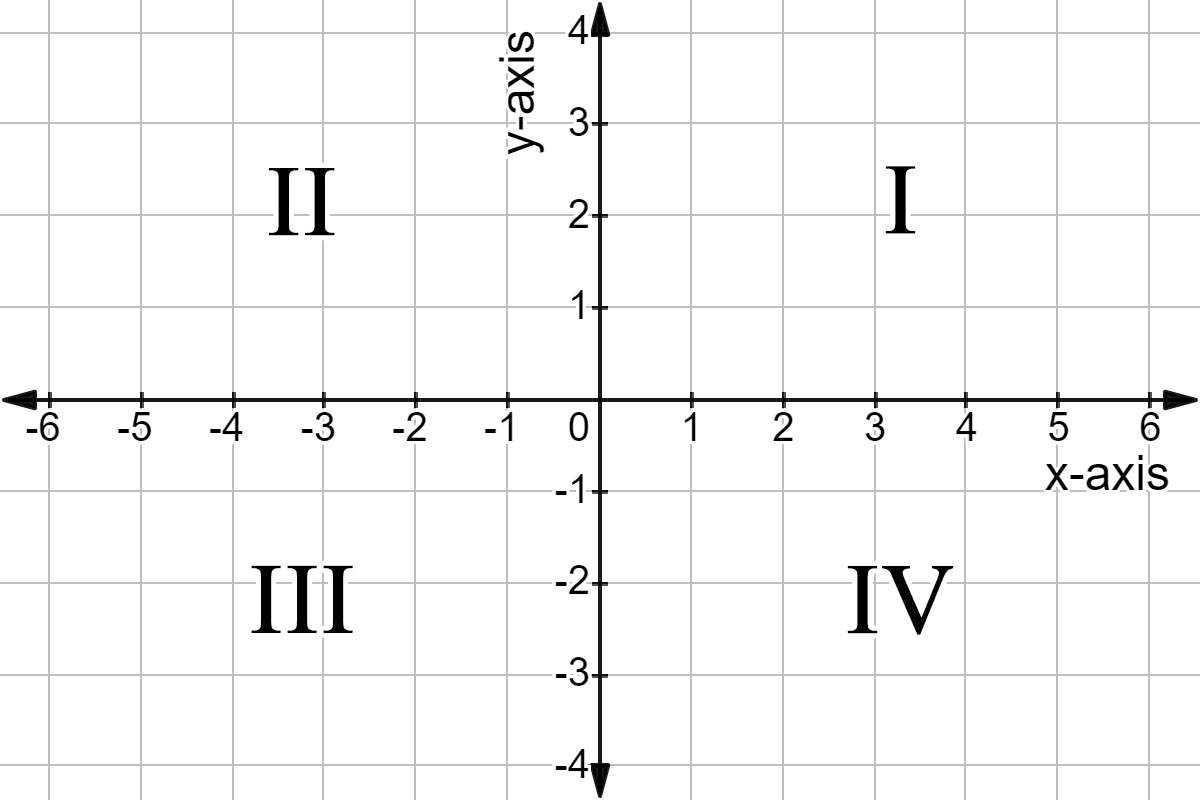
\includegraphics[scale =0.15]{PreCalcPictures/Cartesian Coordinate system.jpg}}
Points on the graph are denoted by $(x,y)$ and are called an ordered pair. Depending on if $x$ and $y$ are positive or negative, they will be positioned in different quadrants.\\
$(x,y)\rightarrow$QI\\
$(-x,y)\rightarrow$QII\\
$(-x,-y)\rightarrow$QIII\\
$(x,-y)\rightarrow$QIV\\
When graphing equations on the coordinate plane, the dependent variable will usually be on the x-axis and the independent variable will be displayed on the y-axis.

\subsubsection{Domain and Range}
Domain is the set of all elements that make up the x-coordinates.\\
Range is the set of all elements that make up the y-coordinates.\\
The domain and range can be expressed in multiple ways:
\begin{itemize}
    \item Inequality Description: $a<x<b$\\
    This means that x is greater than $a$ and less than $b$.
    \item Interval Notation: $x\in (a,b)$\\
    This means that $x$ is between $a$ and $b$, not including $a$ or $b$. If we use square brackets, $x\in [a,b]$, then it means $x$ is between $a$ and $b$ while including $a$ and $b$.\\
    Note that $\infty$ and $-\infty$ will always use round parentheses
    \item Set Notation: $\{x|a<x<b,x\in\mathbb{R}\}$\\
    This translates to the set of $x$ for which $x$ is greater than $a$ and less then $b$ for where $x$ is an element of all real numbers.
\end{itemize}

\subsubsection{Function Definition}
A function is a special type of relation where each element in the domain is associated with exactly one element in the range. (Every x-value can only have one associated y-value).\\
We can determine if a graph is a function or not using the vertical line test. If you move a vertical line along the graph, the line should intersect no more than one point on the curve.\\
Function notation, $f(x)$, is used to denote the result after some operation on the independent variable. $f(x)$ and $y$ are used somewhat interchangeably.